\section{Análisis del estado de máxima entropía}

\subsection{Factorizabilidad}

Nótese que el argumento de la exponencial en la ecuación (\ref{eq:MaxEntLagMult}) está conformado por operadores que conmutan entre sí:
\begin{equation}
    \sum_{j=1}^{3}\lambda_{j}\hat{G}_{j}=\sum_{j=1}^{3}\lambda_{j}\sum_{k=1}^{n}p_{k}(\Id_{2^{k-1}}\otimes\sigma_{j}\otimes\Id_{2^{n-k}}).\nonumber
\end{equation}
Esto significa que el estado de máxima entropía es factorizable y tiene exactamente $n$ factores. Explícitamente,
\begin{equation}\label{eq:MaxEntSeparable}
    \varrho_{\max}=\Motimes_{k=1}^{n}\frac{1}{Z_{k}}\text{exp}\qty(p_{k}\sum_{j=1}^{3}\lambda_{j}\sigma_{j}).
\end{equation}

¿Por qué el estado de máxima entropía resulta ser factorizable respecto a todas las partículas del sistema microscópico? Para responder a esta pregunta, primero hace falta ver que la información accesible al experimentalista no incluye las correlaciones entre los subsistemas. Para ver esto, considérese la parametrización de Bloch de un estado fino $\varrho\in\mcL(sa\hilbert_{4})$ como propuesta en (\ref{eq:BlochParametrization4}). Esto es,
\begin{align}\label{}
    \varrho=\frac{1}{4}\sum_{j,k=0}^{3}\gamma_{jk}\sigma_{i}\otimes \sigma_{k} & & \text{con} & & \gamma_{jk}=\Tr(\sigma_{j}\otimes \sigma_{k}\varrho).\nonumber
\end{align}
De acuerdo con la ecuación (\ref{eq:Ch1PartialTrace}) las matrices de densidad reducidas de $\varrho$ en términos de los parámetros $\gamma_{jk}$ son
\begin{align}
    \rho_{1}=\frac{1}{2}\sum_{j=0}^{3}\gamma_{0j}\pauli{j} & & \text{y} & & \rho_{2}=\frac{1}{2}\sum_{j=0}^{3}\gamma_{j0}\pauli{j}.\nonumber
\end{align}
La matriz de densidad reducida contiene la información estadística de dicho subsistema. Esto significa que las correlaciones entre los subsistemas están contenidas en los elementos $\gamma_{jk}$ tales que $j,k\neq 0$ (los elementos no presentes en las matrices de densidad reducidas). Ahora, la acción de la aplicación de grano grueso sobre la matriz de densidad es justamente
\begin{align}
    \CG{\varrho}&=\Tr_{2}\qty[(p \varrho + (1-p)S\varrho S]\nonumber\\
    &=p\rho_{1}+(1-p)\rho_{2}\nonumber\\
    &=\frac{1}{2}\qty(\Id+\sum_{k=1}^{3}(p\gamma_{k0}+(1-p)\gamma_{0k})\sigma_{k}).\nonumber
\end{align}
¡El estado efectivo no contiene información sobre las correlaciones del estado subyacente! Una consecuencia de esto es que todos los estados pertenecientes a un conjunto de estados microscópicos cuyas matrices de densidad reducidas coinciden tienen la misma imagen bajo la aplicación de grano grueso. Matemáticamente, si se tienen dos estados microscópicos, $\varrho_{A}$ y $\varrho_{B}$, y estos estados cumplen que
\begin{align}
    \Tr_{2}[\varrho_{A}]=\rho_{1} & & \Tr_{1}[\varrho_{A}]=\rho_{2} & & \text{y} & &\Tr_{2}[\varrho_{B}]=\rho_{1} & & \Tr_{1}[\varrho_{B}]=\rho_{2},\nonumber
\end{align}
entonces
\begin{align}
    \CG{\varrho_{A}}=\CG{\varrho_{B}}.\nonumber
\end{align}
Como el estado de máxima entropía respeta el hecho de que no tenemos acceso a las correlaciones, todas ellas, contenidas en los elementos $\gamma_{jk}$ tales que $j,k\neq 0$ se hacen cero \footnote{Es importante señalar que esto no implica que las entradas $\gamma_{jk}$ tales que $j,k\neq 0$ de un estado de máxima entropía $\varrho_{\max}\in\mcL(\hilbert_{4})$ sean nulas (basta con desarrollar la expresión (\ref{eq:MaxEntSeparable}) para ver que no es así), si no que las correlaciones contenidas en dichos elementos son nulas, esto es $\gamma_{jk}=\gamma_{0k}\gamma_{j0}$.}. 


\acnote{Párrafo iterado: notas}

La expresión (\ref{eq:MaxEntSeparable}) es un producto tensorial de $n$ operadores de densidad, a los que denotaremos como $\rho_{j}$, con $\rho_{j}\in\mcL(\hilbert_{2})$. Aún más, nótese que si definimos al vector unitario $\hat{\lambda}$ a través de
\begin{equation}
    \hat{\lambda}_{i}=\frac{\lambda_{i}}{\lambda},\nonumber
\end{equation}
con $\lambda$ dada por la ecuación (\ref{eq:Ch2LagrangeNorm}), entonces todos los factores pueden reescribirse como la exponencial real de $\lambda(\paulivec{\lambda})$ pesado por un factor probabilístico. Ahora, en virtud de la relación (\ref{ap:PauliRealExp}) hallamos
\begin{equation}
    \rho_{j}=\frac{1}{Z_{j}}\qty(\Id\cosh{p_{j}\lambda}+\paulivec{\lambda}\sinh{p_{j}\lambda}).\nonumber
\end{equation}
Para que las matrices reducidas representen estados válidos, las funciones de partición $Z_{j}$ deben valer
\begin{equation}
    Z_{j}=2\cosh{p_{j}\lambda}.\nonumber
\end{equation}
Las matrices de densidad reducidas del estado de máxima entropía tienen la forma
\begin{equation}\label{eq:rhoArhoB}
    \rho_{j}=\frac{1}{2}\qty(\Id+\paulivec{\lambda}\tanh{p_{j}\lambda}).
\end{equation}

\subsection{La relación entre multiplicadores y mediciones}

\acnote{Mediciones? Promedios?}

\acnote{Párrafo iterado: notas}

El problema de la ecuación (\ref{eq:MaxEntSeparable}) es que el estado de máxima entropía está en términos de los multiplicadores de Lagrange, en lugar de cantidades con un significado físico claro. Si por alguna razón tuviéramos que resignarnos a trabajar con el estado en términos de los $\lambda_{i}$, será necesario conocer la expresión del estado macroscópico. Para hallarla, basta con pasar al estado de máxima entropía por la aplicación de grano grueso. Por construcción 
\begin{equation}
    \rho_{\ef}=\CG{\varrho_{\max}}=\sum_{j=1}^{n}p_{j}\rho_{j}.\nonumber
\end{equation}
Sustituyendo las fórmulas de $\rho_{j}$, obtenemos al estado grueso en términos de los multiplicadores de Lagrange.
\begin{equation}\label{eq:CG(MaxEnt)}
    \rho_{\ef}=\frac{1}{2}\qty[\Id+(\paulivec{\lambda})\qty(\sum_{j=1}^{n}p_{j}\tanh(p_{j}\lambda))].
\end{equation}
Pues bien, el estado efectivo tiene su propia parametrización de Bloch. Sea $\vec{r}_{\ef}$ el vector de Bloch de la partícula efectiva. Entonces es claro que
\begin{align}
    r_{\ef}=\sum_{j=1}^{n}p_{j}\tanh(p_{j}\lambda) && \text{y} && \hat{r}_{\ef}=\hat{\lambda},\nonumber
\end{align}
que no son más que la norma y dirección del vector de Bloch del estado efectivo en términos de $\lambda$. De esta manera deducimos la relación entre los promedios de las observables a nivel grueso $\expval{\pauli{j}}=r_{\ef}(\hat{r}_{\ef})_{j}$ y los multiplicadores de Lagrange introducidos para la maximización de la entropía, y es
\begin{equation}
    \expval{\pauli{j}}=\frac{\lambda_{j}}{\lambda}\rfroml(\lambda).
\end{equation}
donde $\rfroml(\lambda)$ es la función que aparece en las ecuaciones (\ref{eq:MaxEntExpVals}),
\begin{equation}\label{eq:r(lambda)}
    \rfroml(\lambda)=\sum_{j=1}^{n}p_{j}\tanh(p_{j}\lambda)
\end{equation}
Ahora, la ecuación (\ref{eq:r(lambda)}), fijadas $p_{j}$, es una suma de $n$ funciones inyectivas, y como tal, es inyectiva también. Esto significa que existe la función inversa. La figura \ref{fig:r(lambda)} muestra la forma de $\rfroml(\lambda)$ para valores selectos de $p_{1}$ en el caso en que $n=2$. Después de una breve inspección de (\ref{eq:r(lambda)}) se concluye que los estados puros corresponden al caso límite $\lambda\rightarrow+\infty$.
Cada multiplicador de Lagrange queda determinado de forma única a través de cantidades experimentales según 
\begin{equation}
    \lambda_{i}=\rfroml^{-1}(r_{\ef}) \frac{\expval{\pauli{i}}}{r_{\ef}},
\end{equation}
y, por supuesto,
\begin{equation}
    \lambda=\rfroml^{-1}(r_{\ef})\nonumber
\end{equation}
Aunque siempre exista, no es posible hallar una expresión de $\rfroml^{-1}$ para cualquier valor de $p$ debido a que la ecuación (\ref{eq:r(lambda)}) es una ecuación trascendental. Por esto, para escribir al estado de máxima entropía como una función de cantidades medibles, nos tendremos que conformar con llamar a $\rfroml^{-1}$ de manera explícita.
\begin{figure}[ht!]
    \centering
    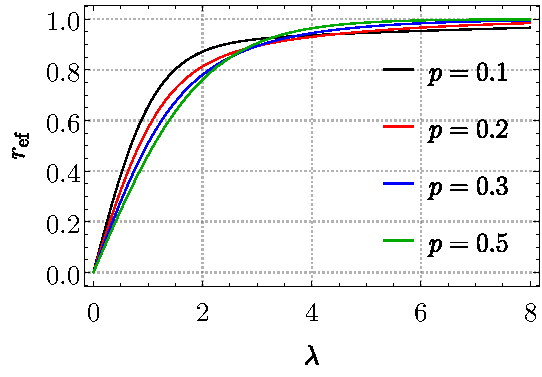
\includegraphics[width=0.5\linewidth]{chapter3/figures/r(lambda).pdf}
    \caption{$r_{\ef}$ como función de $\lambda$ para diferentes valores de $p_{1}$ en el caso en que $n=2$.}
    \label{fig:r(lambda)}
\end{figure}

\subsection{Otra expresión del estado de máxima entropía}

\acnote{Al final nunca usé esto, ¿se queda?}

La ecuación (\ref{eq:MaxEntSeparable}) sugiere que el estado de máxima entropía puede expresarse como producto tensorial de potencias de un mismo estado. En efecto, dado un real $q$ y una matriz cuadrada $A$, la potenciación $A^{q}$ puede escribirse como $e^{q \ln A}$. Como las matrices $e^{\sum_{i}\lambda_{i}\pauli{i}}$ son positivas semidefinidas, su logaritmo es único en el caso de no ser degenerado, y en caso de degeneración, basta con tomar la rama principal \cite{log1,Davalos2019}. Entonces,
\begin{equation}
    \varrho_{\max}=\Motimes_{j=1}^{n}\frac{1}{Z_{j}}e^{p_{j}\sum_{k}\lambda_{k}\pauli{k}}=\Motimes_{j=1}^{n}\frac{1}{Z_{j}}\qty(e^{\sum_{k}\lambda_{k}\pauli{k}})^{p_{j}}.\nonumber
\end{equation}
En virtud de (\ref*{ap:PauliRealExp}), se cumple que
\begin{align}
  \varrho_{\max}=&\Motimes_{j=1}^{n}\frac{\qty(\cosh{\lambda}(\Id+\tanh{\lambda}(\paulivec{r_{\rho}})))^{p_{j}}}{\Tr[\qty(\cosh{\lambda}(\Id+\tanh{\lambda}(\paulivec{r_{\rho}})))^{p_{j}}]}\nonumber\\
  =&\Motimes_{j=1}^{n}\frac{\qty(\Id+\tanh{\lambda}(\paulivec{r_{\rho}}))^{p_{j}}}{\Tr[\qty(\Id+\tanh{\lambda}(\paulivec{r_{\rho}}))^{p_{j}}]}.\nonumber
\end{align}
Definimos
\begin{equation}\label{eq:Xi}
  \Xi_{\max}=\frac{1}{2}(\Id+\tanh{\lambda}(\paulivec{r_{\rho}})),
\end{equation}
de tal manera que 
\begin{equation}\label{eq:MaxEntSeparablePower}
  \varrho_{\max}=\Motimes_{j=1}^{n}\frac{(\Xi_{\max})^{p_{j}}}{\Tr[ (\Xi_{\max})^{p_{j}}]}.
\end{equation}

\subsection{La asignación de máxima entropía}

El estado de máxima entropía nos otorga una herramienta de asignación para los estados efectivos. Después de todo, requerimos de una asignación razonable que pueda ser propagada según la dinámica microscópica conocida. Sea $\rho_{\ef}\in\densityspace{2}$ un estado efectivo, entonces definimos a la aplicación de asignación de máxima entropía como
\begin{equation}\label{eq:MaxEntAss}
    \begin{gathered}
        \mcA_{\mcC}^{\max}:\densityspace{2}\rightarrow\densityspace{2^{n}}\nonumber\\
        \rho_{\ef} \mapsto \Motimes_{j=1}^{n}\frac{1}{Z_{j}}\text{exp}\qty(p_{j}\sum_{k=1}^{3}\lambda_{k}\sigma_{k}).
    \end{gathered}
\end{equation}
donde la dependencia de la asignación en el modelo de grano grueso se indica mediante un subíndice, $\mcC$, ver ecuación (\ref{eq:CG}). Nótese que según los valores que puedan tomar las diferentes probabilidades $p_{j}$, el estado asignado tendrá diferentes propiedades. Nos concentramos en dos casos particulares. El primero corresponde a $p_{1}=1$. En este caso se eliminan los términos de error, y el estado de máxima entropía es simplemente
\begin{equation}\label{eq:PreferentialAss}
    \varrho_{\max}=\rho_{\ef}\otimes\Id^{2^{n-1}},
\end{equation}
Nótese que la aplicación de asignación se vuelve lineal si no hay error de medición. Esto debe verse como un caso límite. Este trabajo estudiará $p_{1}\rightarrow 1$ como el escenario en el que la probabilidad de detectar la partícula equivocada es pequeña. De acuerdo con esto, se le llamará  \textit{regimen de partícula preferencial}.

Ahora, si por otro lado, $p_{j}=\frac{1}{n}\forall j$, entonces el estado de máxima entropía es
\begin{equation}
    \varrho_{\max}=\qty[\frac{1}{Z}\text{exp}\qty(\frac{1}{n}\sum_{k=1}^{3}\lambda_{k}\sigma_{k})]^{\otimes n}=(\rho')^{\otimes n}.\nonumber
\end{equation}
Si se pasa este estado por la aplicación de grano grueso correspondiente el resultado es 
\begin{equation}
    \mcC[\varrho_{\max}]=\sum_{j=1}^{n}\frac{1}{n}\rho'=\rho',\nonumber
\end{equation}
de  lo que se concluye que
\begin{equation*}
    \rho'=\rho_{\ef},
\end{equation*}
y que por lo tanto el estado asignado es simplemente
\begin{equation}\label{eq:BoltzmannAss}
    \mcA_{\mcC}^{\max}(\rho_{\ef})=\rho_{\ef}^{\otimes n}.
\end{equation}
Así, si $p_{j}=\frac{1}{n}\forall j$, la asignación de máxima entropía resulta en un estado factorizable de $n$ partículas idénticas. A este caso se le llamará \textit{régimen imparcial}.



Ahora supóngase que $\varrho$ es un estado microscópico compatible con un estado efectivo puro $\rho_{\ef}=\dyad{\psi}$, y que $p_{j}\neq 0\,\forall\,j$. Entonces, por (\ref{eq:CG}) se cumple que
\begin{equation}
    \rho_{ef}=\sum_{k=1}^{n}p_{k}\varrho_{k},\nonumber
\end{equation}
donde $\varrho_{k}\in\densityspace{2}$ es la $k$-ésima traza parcial de $\varrho$. Como se mencionó en la sección \ref{subsec:ch2_purity}, un estado puro es un punto extremo del conjunto de estados, así que la ecuación anterior solo se puede cumplir si $\varrho_{k}=\dyad{\psi}\,\forall\,k$.  Si cada traza parcial de $\varrho$ es igual al estado puro $\rho_{\ef}$ se sigue que
\begin{equation}\label{eq:PureEffectiveState}
    \varrho=(\rho_{\ef})^{\otimes n}.
\end{equation}
Nótese que para obtener (\ref{eq:PureEffectiveState}) no se hizo ninguna suposición sobre la aplicación de asignación. Lo que se acaba de demostrar es que, dado que todas las trazas parciales participen en la aplicación de grano grueso, el único estado microscópico compatible con un estado efectivo puro es el $n$-producto de dicho estado. El estado (\ref{eq:PureEffectiveState}) es un estado coherente de espín.
